\section{Experiment}

\subsection{Output voltage of a voltage source}

The first experiment featured measurements of the output voltage of a voltage source. The meter was connected to the voltage source in parallel, as shown in Figure~\ref{fig:voltage_schematic}, and measurements were taken for different resistance values.

\begin{figure}[H]
	\centering
	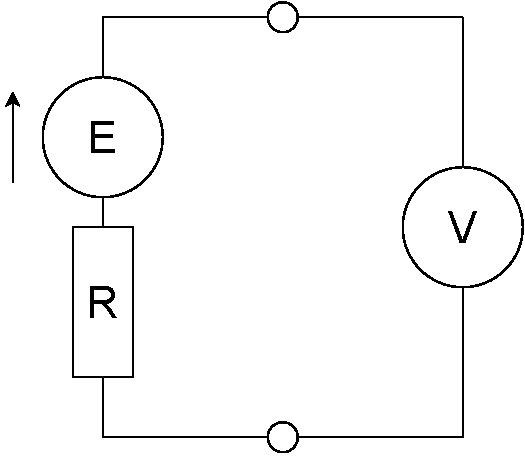
\includegraphics[width=6cm]{schematics/analog_voltage.pdf}
	\caption{Voltage measurements schematic}
	\label{fig:voltage_schematic}
\end{figure}

\subsubsection*{Analog measurements}

The voltmeter that we used for analog measurements is characterized by a 0.5 accuracy class and a  \SI{1}{\frac{\kilo\ohm}{\volt}} internal resistance.
 
 The measurements along with the results are split into Tables~\ref{tab:analog_volt_1} and~\ref{tab:analog_volt_2}; Tab.~\ref{tab:analog_volt_1} contains the measurement results with only the limiting error applied, whereas Tab.~\ref{tab:analog_volt_2} shows the final results which include the systematic error.

\begin{table}[H]
	\centering
	\begin{tabular}{ c | c | c | c | c | c | c | c}
		$R_c [\unit{\ohm}]$ & $\alpha$ & $\alpha_{max}$  & $V_r [\unit{\volt}]$ & $V [\unit{\volt}]$ & $\Delta V [\unit{\volt}]$ & $\delta V  [\unit{\percent}]$ & $V \pm \Delta V [\unit{\volt}]$\\
		\hline
		0 & 40 & 75 & 7.5 & 4.0 & 0.037500 & 0.937500 & $4.00 \pm 0.04$\\
		\hline
		10 & 40 & 75 & 7.5 & 4.0 & 0.037500 & 0.937500 & $4.00 \pm 0.04$\\
		\hline
		100 & 39.5 & 75 & 7.5 & 3.95 & 0.037500 & 0.949367 & $3.95 \pm 0.04$\\
		\hline
		1000 & 35 & 75 & 7.5 & 3.5 & 0.037500 & 1.071429 & $3.50 \pm 0.04$\\
		\hline
		5000 & 56 & 75 & 0.15 & 0.112 & 0.000750 & 0.669643 & $0.1120 \pm 0.0008$\\
		\hline
		10000 & 30 & 75 & 0.15 & 0.06 & 0.000750 & 1.250000 & $0.0600 \pm 0.0008$
	\end{tabular}
	\caption{Analog voltage measurements for $E \sim \SI{3.9}{\volt}$ ($R_c$ -- circuit resistance, $\alpha$ -- actual needle swing, $\alpha_{max}$ -- maximal swing, $V_r$ -- range, $V$ -- measured voltage, $\Delta V$ -- absolute error, $\delta V$ -- relative error)}
	\label{tab:analog_volt_1}
\end{table}

\begin{table}[H]
	\centering
	\begin{tabular}{ c | c | c | c | c | c}
		$R_v [\unit{\ohm}]$  & $\Delta_m V [\unit{\volt}]$ & $\delta_m V $ & $c [\unit{\volt}]$ & $V_c [\unit{\volt}]$ & $V_c \pm \Delta V [\unit{\volt}]$\\
		\hline
		7500 & 0 & 0 & 0 & 4 & 4.00 +- 0.04\\
		\hline
		7500 & -0.005333 & -0.001332 & 0.005333 & 4.005333 & $4.01 \pm  0.04$\\
		\hline
		7500 & -0.052667 & -0.013158 & 0.052667 & 4.002667 & $4.01 \pm 0.04$\\
		\hline
		7500 & -0.466667 & -0.117647 & 0.466667 & 3.966667 & $3.97 \pm 0.04$\\
		\hline
		150 & -3.733333 & -0.970874 & 3.733333 & 3.845333 & $3.8453 \pm 0.0008$\\
		\hline
		150 & -4 & -0.985222 & 4 & 4.06 & $4.0600 \pm 0.0008$
	\end{tabular}
	\caption{Analog voltage measurements for $E \sim \SI{3.9}{\volt}$ ($R_v$ -- internal voltmeter resistance, $\Delta_m V$ -- systematic error, $\delta_m V$ -- ?, $c$ -- correction factor, $V_c$ -- calculated voltage)}
	\label{tab:analog_volt_2}
\end{table}

Example calculations for $R_c = \SI{100}{\ohm} $ are shown in the equations below. %Equations~\ref{eq:analog_V},~\ref{eq:analog_Delta_V},~\ref{eq:analog_delta_V},~\ref{eq:analog_R_v},~\ref{eq:analog_Delta_m},~\ref{eq:analog_delta_m},~\ref{eq:analog_c},~\ref{eq:analog_V_c}.

\begin{equation}
	 V = \frac{\alpha\cdot V_{r}}{\alpha_{max}} = \frac{39.5\cdot \SI{7.5}{\volt}}{75} = \SI{3.95}{\volt}
	 \label{eq:analog_V}
\end{equation}

\begin{equation}
	\Delta V = \frac{V_{r}\cdot cl}{100\unit{\percent}} = \frac{\SI{7.5}{\volt}\cdot 0.5\unit{\percent}}{100 \unit{\percent}} = \SI{0.0375}{\volt}
	\label{eq:analog_Delta_V}
\end{equation}

\begin{equation}
	  \delta V = \frac{\Delta V}{V}\cdot 100\unit{\percent} = \frac{0.0375}{3.95}\cdot 100\unit{\percent} \approx 0.949367\unit{\percent}
	  \label{eq:analog_delta_V}
\end{equation}

\begin{equation}
	R_v = V_r\cdot x = \SI{7.5}{\volt}\cdot \SI{1000}{\frac{\ohm}{\volt}} = \SI{7500}{\ohm}
	\label{eq:analog_R_v}
\end{equation}

\begin{equation}
	\Delta_m V = -V\cdot\frac{R_c}{R_v} = -\SI{3.95}{\volt}\cdot\frac{\SI{100}{\ohm}}{\SI{7500}{\ohm}} \approx -\SI{0.052667}{\volt}
	\label{eq:analog_Delta_m}
\end{equation}

\begin{equation}
	\delta_m V = -\frac{R_c}{R_c + R_v} = -\frac{\SI{100}{\ohm}}{\SI{100}{\ohm} + \SI{7500}{\ohm}} \approx -0.013158
	\label{eq:analog_delta_m}
\end{equation}

\begin{equation}
	c = -\Delta_m V = -(-\SI{0.052667}{\volt}) = \SI{0.052667}{\volt}
	\label{eq:analog_c}
\end{equation}

\begin{equation}
	V_c = V + c = \SI{3.95}{\volt} + \SI{0.052667}{\volt} = \SI{4.002667}{\volt}
	\label{eq:analog_V_c}
\end{equation}


\subsubsection*{Digital measurements}

Digital measurements were made using a multimeter. Its internal resistance and accuracy are available in the device manual; for our calculations we chose the least precise accuracy value that is guaranteed to work for one year after device calibration.

 The measurements along with the results are split into Tables~\ref{tab:digital_voltage_1} and~\ref{tab:digital_voltage_2}; Tab.~\ref{tab:digital_voltage_1} contains the measurement results with only the limiting error applied, whereas Tab.~\ref{tab:digital_voltage_2} shows the final results which include the systematic error.

\begin{table}[H]
	\centering
	\begin{tabular}{ c | c |  c | c | c | c | c}
		$R_c [\unit{\ohm}]$  & Accuracy & $V_r [\unit{\volt}]$ & $V [\unit{\volt}]$ & $\Delta V [\unit{\volt}]$ & $\delta V [\unit{\percent}]$ & $V \pm \Delta V [\unit{\volt}]$ \\
		\hline
		0  & $0.0035 + 0.0005$ & 10 & 3.9996 & 0.000190 & 0.004750 & $3.9996 \pm 0.0002$\\
		\hline
		10  & $0.0035 + 0.0005$  & 10 & 3.99953 & 0.000190 & 0.004750 & $3.9995 \pm 0.0002$\\
		\hline
		100  & $0.0035 + 0.0005$  & 10 & 3.99964 & 0.000190 & 0.004750 & $3.9996 \pm 0.0002$\\
		\hline
		1000 &$0.0035 + 0.0005$  & 10 & 3.99931 & 0.000190 & 0.004750 & $3.9993 \pm 0.0002$\\
		\hline
		5000  & $0.0035 + 0.0005$  & 10 & 3.99791 & 0.000190 & 0.004752 & $3.9979 \pm 0.0002$\\
		\hline
		10000 & $0.0035 + 0.0005$  & 10 & 3.99593 & 0.000190 & 0.004751 & $3.9959 \pm 0.0002$\\
	\end{tabular}
	\caption{Digital voltage measurements for $E \sim \SI{3.9}{\volt}$ ($R_c$ -- circuit resistance, Accuracy: $\pm$ (a$\unit{\percent}$ of reading + b$\unit{\percent}$ of range), $V_r$ -- range, $V$ -- measured voltage, $\Delta V$ -- absolute error, $\delta V$ -- relative error)}
	\label{tab:digital_voltage_1}
\end{table}

\begin{table}[H]
	\centering
	\begin{tabular}{  c | c | c | c | c | c}
		 $R_v [\unit{\mega\ohm}]$ & $\Delta_m V [\unit{\volt}]$ & $\delta_m V$ & $c [\unit{\volt}]$ & $V_c [\unit{\volt}]$ & $V_c \pm \Delta V [\unit{\volt}]$\\
		\hline
		10 & 0 & 0 & 0 & 3.9996 & $3.9996 \pm 0.0002$\\
		\hline
		10 & -0.000003 & -0.000001 & 0.000004 & 3.999534 & $3.9995 \pm 0.0002$\\
		\hline
		10 & -0.000040 & -0.000010 & 0.000040 & 3.999680 & $3.9997 \pm 0.0002$\\
		\hline
		10 & -0.000400 & -0.000100 & 0.000400 & 3.999710 & $3.9997 \pm 0.0002$\\
		\hline
		10 & -0.001999 & -0.000500 & 0.001999 & 3.999909 &$ 3.9999 \pm 0.0002$\\
		\hline
		10 & -0.003996 & -0.000999& 0.0039969 & 3.999926 & $3.9999 \pm 0.0002$\\
	\end{tabular}
	\caption{Digital voltage measurements for $E \sim \SI{3.9}{\volt}$ ($R_v$ -- internal multimeter resistance, $\Delta_m V$ -- systematic error, $\delta_m V$ -- ?, $c$ -- correction factor, $V_c$ -- calculated voltage)}
	\label{tab:digital_voltage_2}
\end{table}

Example calculations for $R_c = \SI{5000}{\ohm}$ are shown in the equations below. %Equations~\ref{eq:digital_Delta_V},~\ref{eq:digital_delta_V},~\ref{eq:digital_Delta_m},~\ref{eq:digital_delta_m},~\ref{eq:digital_c},~\ref{eq:digital_V_c}.

\begin{equation}
	\begin{split}
		\Delta V &= \frac{a}{100\unit{\percent}}\cdot V + 	\frac{b}{100\unit{\percent}}\cdot V_r = \frac{0.0035\unit{\percent}}{100\unit{\percent}}\cdot\SI{3.99791}{\volt} + \frac{0.0005\unit{\percent}}{100\unit{\percent}}\cdot\SI{10}{\ohm} =\\
		&= \SI{0.00014}{\volt} + \SI{0.00005}{\volt} = \SI{0.00019}{\volt}
	\end{split}
	\label{eq:digital_Delta_V}
\end{equation}

\begin{equation}
	\delta V = \frac{\Delta V}{V}\cdot 100\unit{\percent} = \frac{\SI{0.00019}{\volt}}{\SI{3.99791}{\volt}}\cdot 100\unit{\percent} = 0.004752\unit{\percent}
	\label{eq:digital_delta_V}
\end{equation}

\begin{equation}
	\Delta_m V = -V\cdot\frac{R_c}{R_v} = -\SI{3.99791}{\volt}\cdot\frac{\SI{5000}{\ohm}}{\SI{10000000}{\ohm}} \approx -\SI{0.001999}{\volt}
	\label{eq:digital_Delta_m}
\end{equation}

\begin{equation}
	\delta_m V = -\frac{R_c}{R_c + R_v} = -\frac{\SI{5000}{\ohm}}{\SI{5000}{\ohm} + \SI{10000000}{\ohm}} \approx -0.000500
	\label{eq:digital_delta_m}
\end{equation}

\begin{equation}
	c = -\Delta_m V = -(-\SI{0.001999}{\volt}) = \SI{0.001999}{\volt}
	\label{eq:digital_c}
\end{equation}

\begin{equation}
	V_c = V + c = \SI{3.99791}{\volt} + \SI{0.001999}{\volt} = \SI{3.999909}{\volt}
	\label{eq:digital_V_c}
\end{equation}


\subsection{Voltage divider}

In the second experiment we measured and compared the input and output voltages of a voltage divider. Meters were connected to the circuit in parallel (Figure~\ref{fig:voltage_divider_schematic}).

\begin{figure}[H]
	\centering
	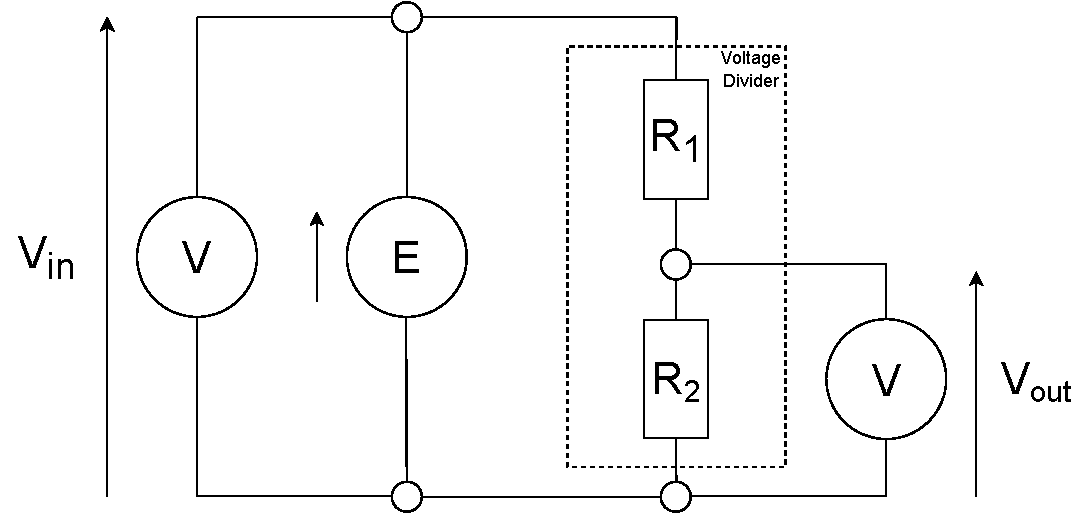
\includegraphics[width=12cm]{schematics/voltage_divider.pdf}
	\caption{Voltage measurements schematic}
	\label{fig:voltage_divider_schematic}
\end{figure}

For each measurement one of the voltages was measured with an analog voltmeter and the other one with a digital multimeter. Measurements were taken for different voltage divider ratio and resistance values.

Table~\ref{tab:voltage_divider} shows all of the measurements along with the results. Precision wasn't the primary focus of this experiment, hence all values have been rounded to one decimal place.

\begin{table}[H]
	\centering
	\begin{tabular}{|c c  c  c  c  c  c  c c  c  c|}
		\hline
		\multicolumn{5}{|c}{\multirow{2}{*}{}} & \multirow{2}{*}{Analog} & \multirow{2}{*}{Digital} & \multicolumn{4}{c|}{ \multirow{2}{*}{ }}\\
		&&&&&&&&&&\\
		\hline
		$k$ &	$R [\unit{\ohm}]$ & 	$\alpha$ & $\alpha_{max}$ &	$V_r [\unit{\volt}]$ & $V_{in} [\unit{\volt}]$ &	$V_{out} [\unit{\volt}]$ & $R_{in}$ [\unit{\ohm}]& $R_{out}$ [\unit{\ohm}]&  $	\frac{V_{out}}{V_{in}}$ & $\Delta_k$\\
		\hline
		0.9	& 1k	& 40 & 75 &	7.5	& 4	& 3.6 &	7.5k &	10M&	0.9	& 0\\
		\hline
		0.5	& 1k	& 40 &	75	& 7.5 &	4 &	2	& 7.5k	& 10M	& 0.5	& 0\\
		\hline
		0.1	& 1k &	40 & 75	& 7.5	& 4 &	0.4&	7.5k &	10M&	0.1 &	0\\
		\hline
		0.9 &	1M &	40 &	75	& 7.5 &	4	& 3.6	& 7.5k&	10M	& 0.9 &	0\\
		\hline
		0.5	& 1M	& 40	& 75 &	7.5 &	4	& 1.9	& 7.5k &	10M &	0.5	& 0\\
		\hline
		0.1	& 1M	& 40	& 75	& 7.5 &4	&0.4 &	7.5k &	10M	& 0.1 &	0\\
		\hline
		\multicolumn{5}{|c}{\multirow{2}{*}{}} & \multirow{2}{*}{Digital} & \multirow{2}{*}{Analog} & \multicolumn{4}{c|}{ \multirow{2}{*}{ }}\\
		&&&&&&&&&&\\
		\hline
		0.9	& 1k & 36 &	75 &	7.5 &	4 & 3.6 &	10M & 	7.5k & 0.9	& 0\\
		\hline
		0.5	& 1k &	44 & 75 & 3	& 4	& 1.8	& 10M &	3k & 0.4 & 0.1\\
		\hline
		0.1	& 1k & 35.5 & 75 & 0.75 & 4 &	0.4 & 	10M &	0.75k &	0.1	& 0\\
		\hline
		0.9	& 1M &	3	& 75	& 0.15	& 4 &	0 &	10M &	0.15k &	0 &	0.9\\
		\hline
		0.5	& 1M & 0.5	& 75	& 0.15 &	4 &	0 &	10M &	0.15k &	0&	0.5\\
		\hline
		0.1 &	1M &	0	& 75 &	0.15 &	4 &	0 &	10M &	0.15k &	0 &	0.1\\
		\hline
	\end{tabular}
	\caption{Voltage measurements for $E\sim\SI{4}{\volt}$ ($k$ -- set divider ratio, $R$ --  equivalent divider resistance, $\alpha$ -- actual needle swing, $\alpha_{max}$ -- maximal swing, $V_r$ -- range, $V_{in}$ -- input voltage, $V_{out}$ -- output voltage, $R_{in}$, $R_{out}$ -- internal meter resistances, $\frac{V_{out}}{V_{in}}$ -- measured divider ratio, $\Delta_k$ -- ratio error)}
	\label{tab:voltage_divider}
\end{table}

Example calculation for $k = 0.9$, $R = \SI{1}{\kilo\ohm}$, $V_{in}$ measured with an analog meter, and $V_{out}$ measured with a digital meter are shown in the equations below.

\begin{equation}
	V_{in} = \frac{\alpha\cdot V_r}{\alpha_{max}} = \frac{40\cdot\SI{7.5}{\volt}}{75} = \SI{4}{\volt}	
\end{equation}

\begin{equation}
	R_{in} = V_r\cdot x = \SI{7.5}{\volt}\cdot \SI{1}{\frac{\kilo\ohm}{\volt}} = \SI{7.5}{\kilo\ohm}
\end{equation}

\begin{equation}
	\frac{V_{out}}{V_{in}} = \frac{\SI{3.6}{\volt}}{\SI{4}{\volt}} = 0.9
\end{equation}

\begin{equation}
	\Delta_k = | k - \frac{V_{out}}{V_{in}}| = |0.9 - 0.9| = 0
\end{equation}